\begin{frame}[t]{Introduction}
	{Background}
	
	\begin{itemize}
		\item <1-> Rudimentary theoretical work on the development of galaxies dates back to the twentieth century on a planet called Earth in galaxy sector GS5281, locally known as the Milky Way galaxy. 
		\item A remarkable achievement, given that the learned ones of the planet seem oblivious to the existence of The Force.
		\item <1-> While these simplistic theories have been useful, unsurprisingly it fails to predict the internal structure and evolution of a vast majority of the galaxies in the observable universe, \item <1-> The Galaxy being one prominent example.
	\end{itemize}
	
	\begin{tikzpicture}[remember picture,overlay]
%	\node (sw) at (page cs:0,0){}; % bottom left
%	\node (se) at (page cs:1,0){}; % bottom right
%	\node (ne) at (page cs:1,1){}; % top    right
%	\node (nw) at (page cs:0,1){}; % top    left
	
	\node <1->(image) at (page cs:0.80,0.25)
	{
		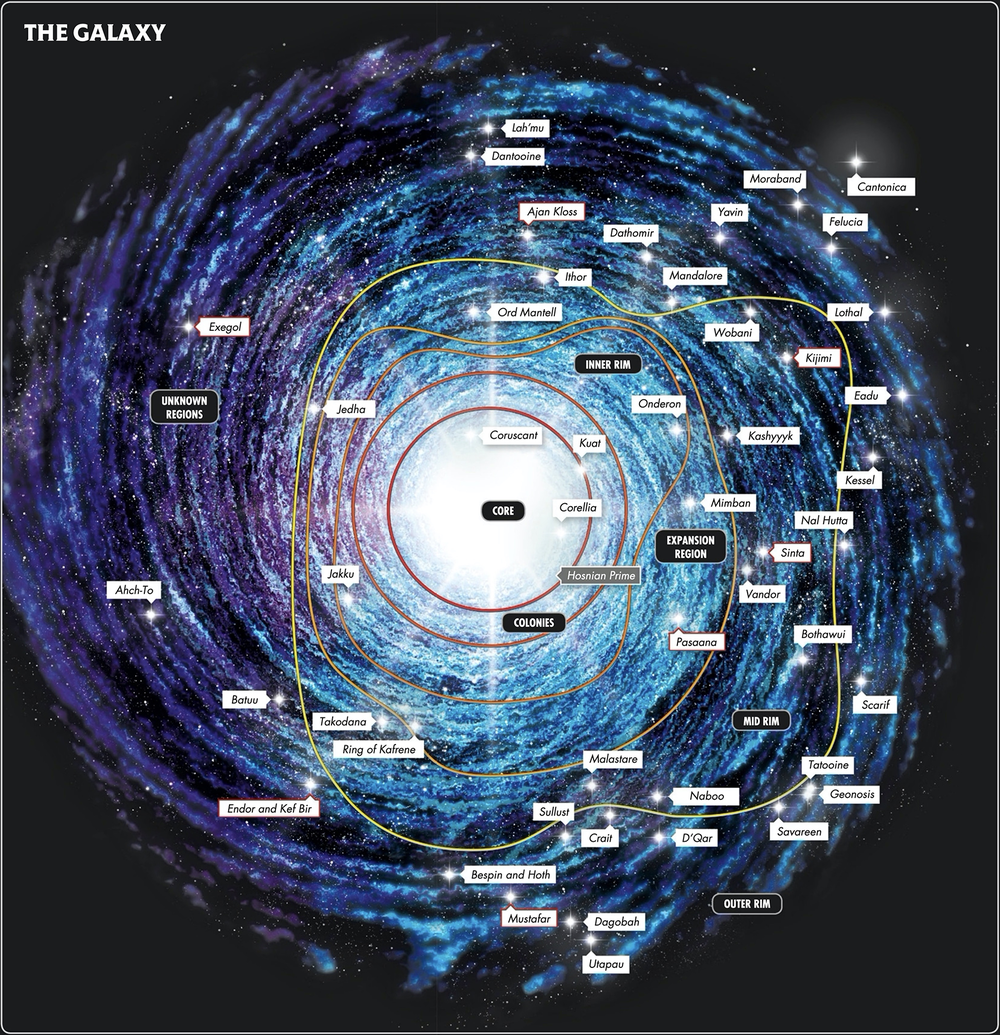
\includegraphics[width=.25\paperwidth]{The_Galaxy_TROS_visual.png}
	};
	
	\end{tikzpicture}
	
\end{frame}
%-------------------------------------------------------------------------------

%-------------------------------------------------------------------------------
